\chapter{组件-事件知识图谱表示学习}
本章主要设计了针对组件-事件知识图谱的知识表示学习模型。在已有的知识库中(如FB15K\cite{bordes2013translatingE}和YAGO37\cite{guo2018knowledge}),由于每个三元组$\left(head, relation, tail\right)$都可以视作一条知识而单独存在,知识图谱可以用多个三元组组成的集合表示,即 $\mathcal{KG}=\left\{\left(e_{i}, r_{k}, e_{j}\right)\right\}$(其中$i$、$j$为实体索引,$k$为关系索引)。因此,已有的大多数知识表示模型都是输入三元组$\left(head, relation, tail\right)$,然后着重于缩短这三者嵌入表示之间的语义距离。

在本文的组件-事件知识图谱$G=(\mathcal{F}, \mathcal{V}, \mathcal{E}, \mathcal{R})$中,每个组件-事件知识图谱都对应着一个故障类型$\mathcal{F}$,这使得每个三元组的成立与其上下文背景信息有关,且每个实体在不同的上下文中应有不同的嵌入表示,即应随着上下文的变化而动态地表示。详细分析如\ref{backgroud-analysis}所示。虽然文献\parencite{feng2016gake,shi2017knowledge}尝试将图结构上下文引入嵌入表示,但是它们都将原本的图结构转为邻居上下文、路径上下文再进行嵌入表示学习。这种方式不足以获取全面的图结构上下文信息,且不能满足动态的嵌入表示学习(不能根据具体上下文给同一实体不同的嵌入表示),所以本文利用图神经网络获取组件-事件知识图谱中的图结构信息,再结合实体的语义信息,获取动态的实体嵌入表示。
\section{场景特性分析}\label{backgroud-analysis}
% GCN  RGCN  SACN KBAT
本节主要分析了组件-事件知识图谱的特性,解释了为何本文的知识表示学习与上下文背景信息相关,且需要动态的嵌入表示。

\subsection{上下文背景信息}\label{context-analysis}
在组件-事件知识图谱中,一个三元组的成立与其上下文拓扑关系有关,这使得一个三元组不能被视为一条可以单独存在的知识。下面是以图\ref{graph-example}中信息为例,对组件-事件知识图谱中三大类关系的分析:

1)事件到事件的因果关系。以三元组$\left(Backoff, cause, HttpServerError Exception 503\right)$为例,该三元组中$Backoff$(微服务重启失败)的发生不一定会导致$HttpServerError 503$(微服务服务不可用)。该三元组的成立,需要一定的背景信息如式\ref{event-event-relation}所示,即需要这两个事件发生在同一个微服务组件、或者有交互依赖关系的两个微服务组件。
\begin{equation}
    \begin{aligned}
        &\left ( ts-train-service, happen, Backoff \right ) \\
        &\wedge \left ( ts-ticketinfo-service, happen, HttpServerError Exception 503 \right ) \\
        &\wedge \left ( ts-ticketinfo-service, call, ts-train-service \right ) \\
        &\Rightarrow \left ( Backoff, \boldsymbol{cause}, HttpServerError Exception 503 \right )
    \end{aligned}
\label{event-event-relation}
\end{equation}

% 1)事件到事件的因果关系。以预测三元组中尾实体$\left(Backoff, cause, \textcolor[rgb]{1,0,0}{?}\right)$为例,推理关系如式\ref{event-event-relation-entity}所示,即需要这两个事件发生在同一个微服务组件、或者有交互关系的两个微服务组件。
% \begin{equation}
%     \begin{aligned}
%         &\left ( ts-train-service, happen, Backoff \right ) \\
%         &\wedge \left ( ts-ticketinfo-service, happen, HttpServerError Exception 503 \right ) \\
%         &\wedge \left ( ts-ticketinfo-service, call, ts-train-service \right ) \\
%         &\Rightarrow \left ( Backoff, \boldsymbol{cause}, HttpServerError Exception 503 \right )
%     \end{aligned}
% \label{event-event-relation-entity}
% \end{equation}

2)组件到事件的发生关系。以三元组$\left( ts-travel-service, happen, HttpServerError Exception 500 \right)$为例,该三元组中$ts-travel-service$是否会发生事件$HttpServerError Exception 500$同样与其周边设备的状态有关。该三元组成立依据于式\ref{event-device-relation}。
\begin{equation}
    \begin{aligned}
        &\left ( ts-ticketinfo-service, happen,  HttpServerError Exception 503\right ) \\
        &\wedge \left ( ts-travel-service, call, ts-ticketinfo-service \right ) \\
        &\wedge \left ( HttpServerError Exception 503, cause, HttpServerError Exception 500 \right ) \\
        &\Rightarrow \left ( ts-travel-service, \boldsymbol{happen}, HttpServerError Exception 500 \right )
    \end{aligned}
\label{event-device-relation}
\end{equation}

3)组件到组件的交互关系。以三元组$\left( container1, hold, ts-train-service \right)$为例,该三元组中$container1$负载着$ts-train-service$而不是其他微服务,同样需要借助背景信息才能推导出来。背景信息推到出该三元组成立如式\ref{device-device-relation}所示。
\begin{equation}
    \begin{aligned}
        &\left ( container1, happen,  cpu 100\% \right ) \\
        &\wedge \left ( container1, happen,  memory 100\% \right) \\
        &\wedge \left ( ts-train-service, happen,  Backoff \right) \\
        &\wedge \left ( cpu 100\%, cause,  Backoff \right) \\
        &\wedge \left ( memory 100\%, cause,  Backoff \right) \\
        &\Rightarrow \left ( container1, \boldsymbol{hold}, ts-train-service \right )
    \end{aligned}
\label{device-device-relation}
\end{equation}

由上述分析可见,组件-事件知识图谱中每条三元组都不能作为一条知识单独存在,而是整个知识图谱中三元组之间相互佐证使得整个拓扑图成为了蕴含知识的知识图谱。由此启发,组件-事件知识图谱的知识表示学习需要将实体所在上下文背景信息考虑进去,才能学习得到有效的实体与关系嵌入表示。
% 在组件-事件知识图谱表示学习中,需要考虑三元组的上下文。
% 已有的方式
% 引入逻辑规则,在传统的知识图谱中,关系都有丰富的语义信息(与常识知识有关),可以根据语义信息生成一些推理规则。比如
% isMarriedTo(x,y)->isMarriedTo(y,x)
% hasChild(x,y)且isCitizenOf(y,z)->isCitizenOd(x,z)
% playsFor(x,y)->isAffiliatedTo(x,y)
% 在组件-事件知识图谱中,只有因果关系,产生关系和交互关系,语义信息不足,生成的规则不具有通用性。规则是否成立其与具体的拓扑关系、抽象事件类型、组件类型都有关系。比如\ref{graph-example}中从“微服务ts-train-service发生BackOff就会导致请求它的微服务ts-ticketinfo-service发生HttpServerError”可以生成规则“微服务x发生BackOff就会导致请求它的微服务y发生HttpServerError”。该条规则只在当前的分布式应用可用,随着应用更新(添加了备用的微服务ts-train-service2或者开发人员添加异常处理使之不报错)或在其他的两个有访问关系的微服务之间,该条规则就会不适用。一方面规则需要大量人工编写审核,一方面即使自动生成规则也没有通用性,所以引入规则进行知识表示学习不可行。
\subsection{动态嵌入表示}
根据\ref{context-analysis}节分析,本文知识图谱表示学习需要引入上下文背景信息。在引入上下文背景信息方面,文献\parencite{feng2016gake,shi2017knowledge}将实体所在的图结构转为邻居上下文、路径上下文,通过最大化实体在其上下文的条件概率进行嵌入表示学习。但这种最大化概率的方式,对实体、关系的嵌入表示是静态的,即一旦训练完成嵌入表示是不会再随着上下文改变的。

这种获取静态嵌入表示的方法不适用于组件-事件知识图谱的表示学习。因为同一抽象事件由于其所在上下文不同、所在设备不同应当有着不同的嵌入表示。如图\ref{order-service-error}所示是"订票服务不可用"故障对应的组件-事件知识图谱部分示意图,在该图中同样存在$Backoff$抽象事件和$\left(ts-travel-service, happen, HttpServiceError Exception 500\right)$三元组,但该图中$ts-travel-service$发生$HttpServiceError Exception 500$是由于订票微服务$ts-order-service$上发生的抽象事件$Backoff$导致的。相对应的图\ref{graph-example}中$ts-travel-service$发生$HttpServiceError Exception 500$是微服务$ts-train-service$上的$Backoff$间接导致的,对应着"数据库不可用无法查票"故障。在这两个故障场景中,抽象事件$HttpServiceError Exception \\500$是由不同原因导致的,所以应有不同的嵌入表示。抽象事件$Backoff$发生在不同的微服务上,也应有着不同的嵌入表示。所以,在组件-事件知识图谱中,实体、关系嵌入表示需要随上下文信息动态变化。
\begin{figure}[htbp]
    \centering
    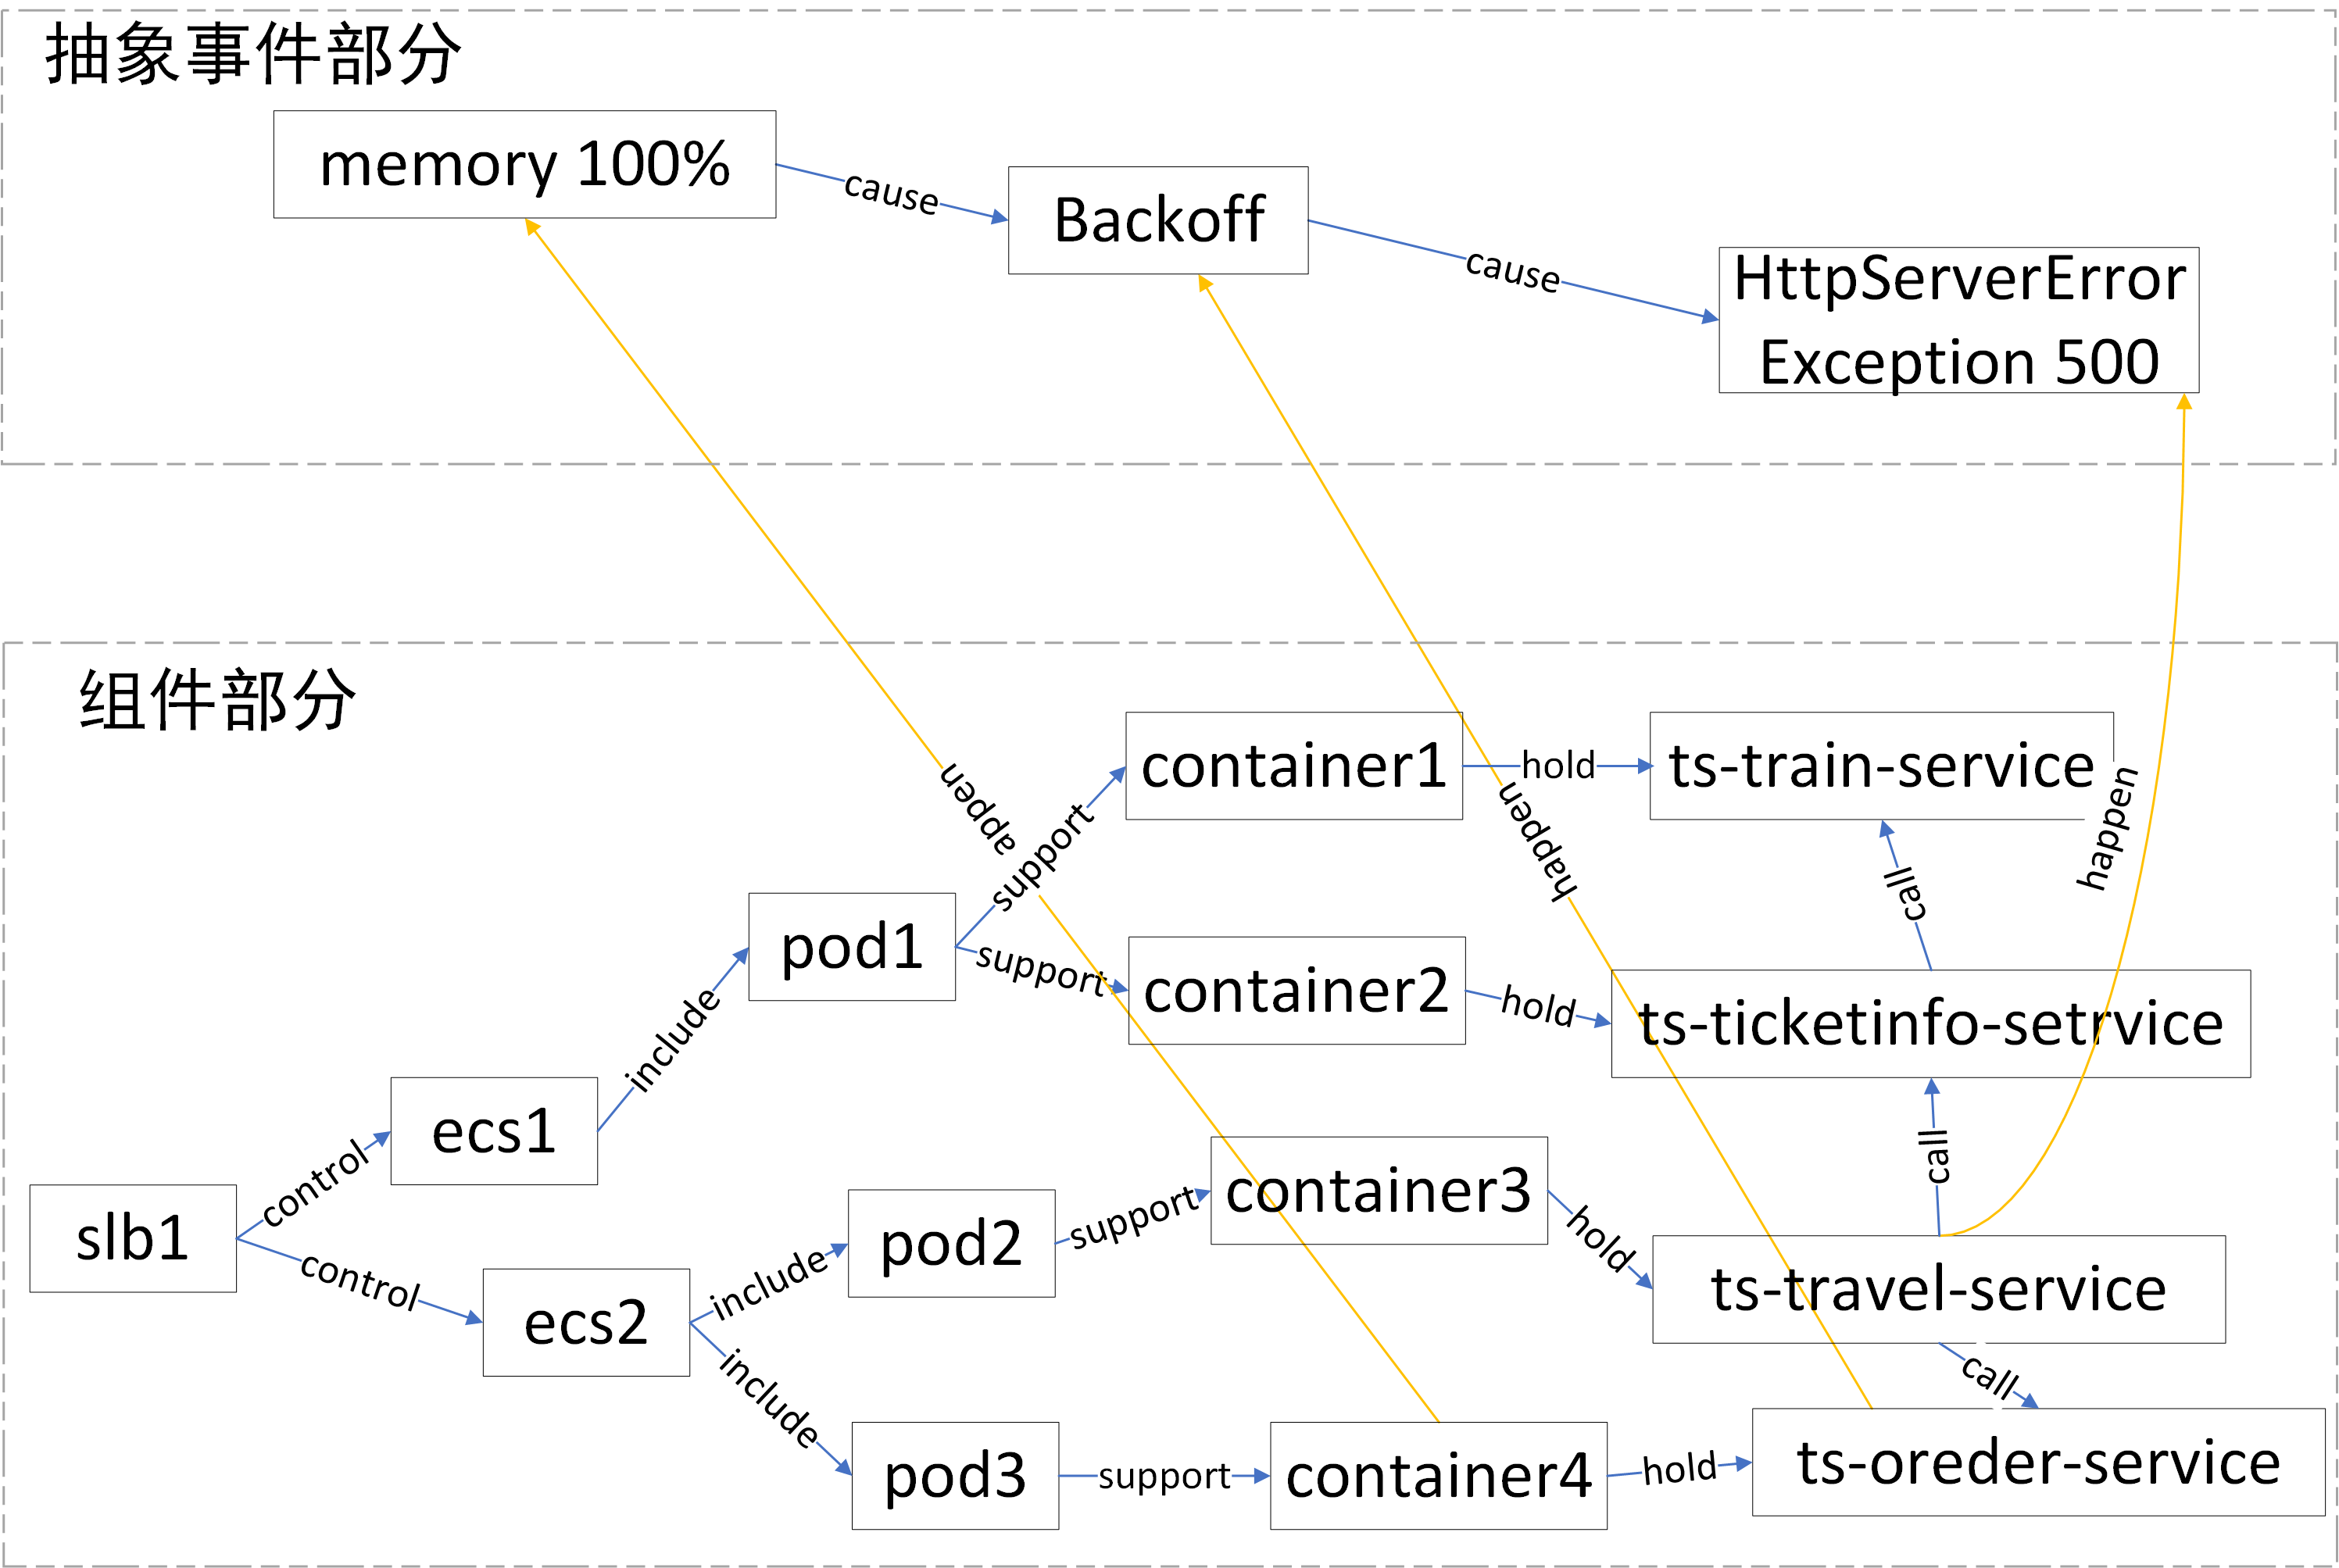
\includegraphics[width=.8\textwidth]{order-service-error.png}
    \caption{订票服务不可用故障对应知识图谱部分示例\label{order-service-error}}
\end{figure}

根据上下文进行动态表示在词嵌入领域已经有大量的相关工作。在最初的工作中,word2vec\cite{mikolov2013efficient}最大化单词在上下文出现的概率,将每个单词表示为低维稠密的静态向量,却忽视了单词在不同上下文含义不同。为了识别单词在不同上下文中具体的语义,ELMo\cite{peters2018deep}提出使用双层记忆网络,Bert\cite{devlin2018bert}使用基于自注意力机制的Transformer\cite{vaswani2017attention}作为编码层以获取单词随上下文变动的动态词向量。其中Bert所使用的Transformer结构其实是将一段文本看做单词为结点的全连接图。受此启发,本文将知识图谱看作稀疏图,使用图卷积网络作为编码器,以引入三元组上下文的图结构信息。本文进一步将图卷积网络获取的上下文图结构信息与三元组实体的文本语义信息融合,从而获取了三元组在不同上下文的动态表示。

% 1.rgcn后面连接的解码器什么样子
% 2.loss函数怎么计算 分类 关系 还是 头尾实体预测
% 3.模型的输入是什么


\section{基于图卷积网络的上下文图结构嵌入算法}\label{RGCN}
本小节介绍文献\parencite{schlichtkrull2018modeling}中基于图卷积网络的RGCN算法,该算法基于图信息传播机制获取了知识图谱中实体关系的上下文图结构信息。
\subsection{模型结构}
嵌入层:该层主要为了引入实体多维度的信息,如实体包含着的各种语义信息。对于每个实体,该文献将其不同的文本属性连接起来,并使用预先训练的Bert模型来获得它们的嵌入表示。这些嵌入表示形成了实体的初始特征向量。对于实体没有属性的数据集,嵌入层则是随机初始化的。

图卷积层:图卷积网络是将局部的信息通过关系传递到整个图中,因此可以将其理解为一个可微分消息传递框架的特例,可以用式子\ref{propo-example}表示。
\begin{equation}
    h_{i}^{(l+1)}=\sigma\left(\sum_{m \in \mathcal{M}_{i}} g_{m}\left(h_{i}^{(l)}, h_{j}^{(l)}\right)\right)
    \label{propo-example}
\end{equation}

$h_{i}^{(l)} \in \mathbb{R}^{d^{(l)}}$是结点$v_{i}$在$l$-th层神经网络的隐状态,$d^{(l)}$是该层隐状态向量的维度。$g_{m}(\cdot, \cdot)$函数计算了$v_{j}$传入结点$v_{i}$的信息。随后累加$v_{i}$每个邻居结点传来的信息,并将累计结果传入激活函数$\sigma(\cdot)$就可以得到$v_{i}$在下一层神经网络的隐状态向量$h_{i}^{(l+1)}$,其中激活函数可以使用$\operatorname{ReLU}(\cdot)=\max (0, \cdot)$等常见的激活函数。$\mathcal{M}_{i}$表示结点$v_{i}$的传入信息集合,其中每一条传入信息都与一条边对应。$g_{m}(\cdot, \cdot)$通常为类似于神经网络的函数或简单的线性变换$g_{m}\left(h_{i}, h_{j}\right)=W h_{j}$,$W$为权重矩阵(如文献\parencite{kipf2016semi}所示)。这样的信息计算函数有效地累计并编码了来自局部的结构化邻域特征,并在诸如图分类\parencite{duvenaud2015convolutional}和图的半监督学习等领域取得了显著的改进效果。

基于上文的消息传递架构,一个知识图谱可以表示为$Graph=\left(\mathcal{V},\mathcal{E},\mathcal{R}\right)$,其中$v_i\in\mathcal{V}$表示结点,$\left(v_i,r,v_j\right)\in\mathcal{E}$表示被标注的边,$r\in\mathcal{R}$表示关系类型。
% 在本文中,$\mathcal{R}$包含正向因果(导致)、反向因果(被导致)两种关系类型。
其信息传播过程如式\ref{propo-in-directedgraph}所示。该式用于计算有向图中由$v_{i}$表示的实体或节点的隐状态随信息传递的变化。
\begin{equation}
    h_{i}^{(l+1)}=\sigma\left(\sum_{r \in \mathcal{R}} \sum_{j \in \mathcal{N}_{i}^{r}} \frac{1}{c_{i, r}} W_{r}^{(l)} h_{j}^{(l)}+W_{0}^{(l)} h_{i}^{(l)}\right)
    \label{propo-in-directedgraph}
\end{equation}
其中,$h_i^{\left(l\right)}\in R^{d^{\left(l\right)}}$为结点$v_i$在第$l$层神经网络的隐状态,$d^{\left(l\right)}$是该层网络表示空间的维度。而$\mathcal{N}_{i}^{r}$是索引为i的结点在关系$r\in\mathcal{R}$下的所有邻接结点索引值集合。$c_{i,r}$是特定于问题的规范化常量,可以被学习或预先指定(例如$c_{i, r}=\left|\mathcal{N}_{i}^{r}\right|$)。该方法通过归一化和来计算相邻节点传播来的信息,并且只选择依赖于相邻结点的线性变换$Wh_j$具有重要的计算优势,既不需要使用大量内存保存关系向量,也通过使用稀疏矩阵乘法减少了资源消耗。

\begin{figure}[htbp]
    \centering
    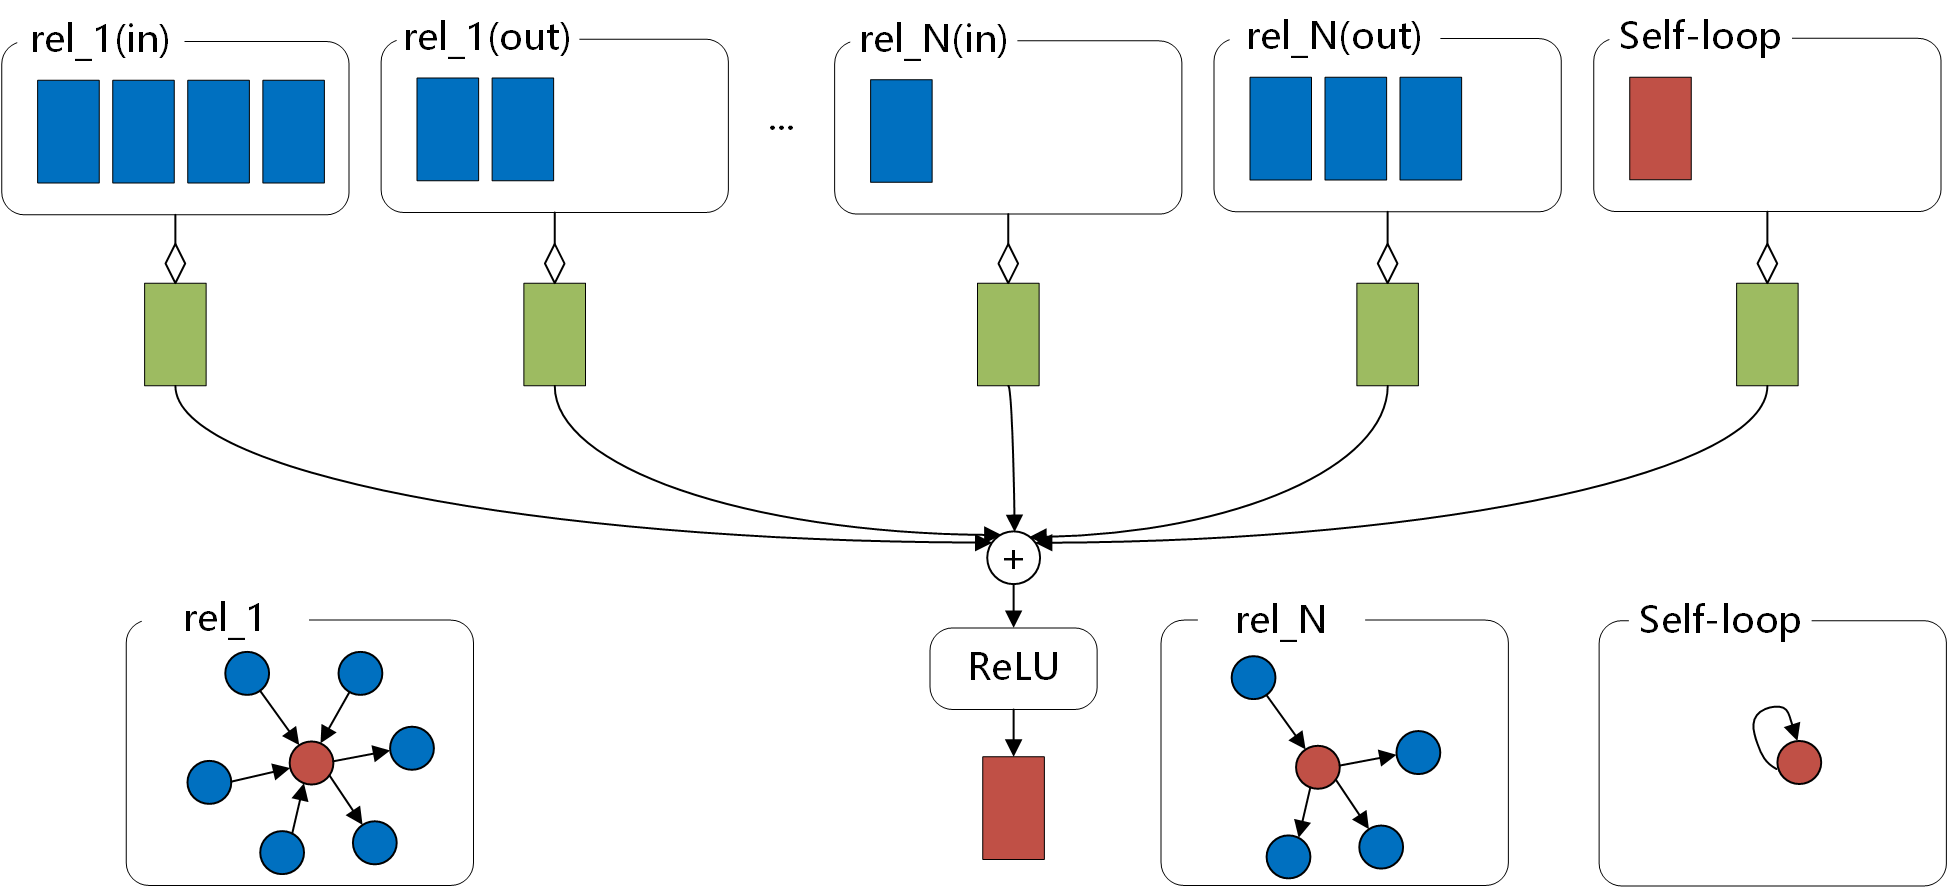
\includegraphics[width=.8\textwidth]{rgcn-cal.png}
    \caption{每层图网络隐状态更新过程\label{rgcn-cal}}
\end{figure}

每一层图网络的更新都需要对有向图中每个节点按照公式\ref{propo-in-directedgraph}进行并行计算。在模型实现中,可以堆叠多个图网络层以实现跨多个关系的依赖关系。其中单个节点更新的计算图如图\ref{rgcn-cal}所示。待更新隐状态的结点/实体为红色,其相邻节点为深蓝色,都用$d$维度的向量表示。然后针对每个关系类型分别进行信息计算,信息计算结果表示(绿色)以标准化和的形式累加,最后经过激活函数(如ReLU)作为新的隐状态向量。

\subsection{模型训练}
模型训练方面主要使用了来自实体分类和链接预测两方面的损失函数。

实体分类:将如式子\ref{propo-in-directedgraph}的每一层图神经网络堆叠起来,并在最后一层节点的输出隐状态向量上使用$\operatorname{softmax}(\cdot)$激活函数。最终在标注的结点上最小化式\ref{node-class-crossenphory}表示的交叉熵损失函数即可。
\begin{equation}
    \mathcal{L}=-\sum_{i \in \mathcal{Y}} \sum_{k=1}^{K} t_{i k} \ln h_{i k}^{(L)}
    \label{node-class-crossenphory}
\end{equation}

其中$\mathcal{Y}$是有标签的结点索引集,$h_{i k}^{(L)}$是索引为$i$的带标签结点对应的网络输出的第$k$维度的值。$t_{i k}$表示该实体的标注向量的第$k$维度的值。最后使用梯度下降算法训练模型参数即可。

链接预测:预测新的事实是否存在(即三元组$(head,relation,tail)$是否存在)。在形式上,知识库可以用一个有方向的、有标注的图表示,即$G=(\mathcal{V}, \mathcal{E}, \mathcal{R})$。训练过程中没有使用完整的边集$\mathcal{E}$,而是使用了其子集$\hat{\mathcal{E}}$。模型会给候选边$(h, r, t)$一个分数$f(h, r, t)$,用以确定该边属于$\mathcal{E}$的可能性有多大。
为了进行链接预测,该文献引入了图编码-解码模型,包含着一个实体编码器和一个评分函数(即解码器)。编码器将每一个实体$v_{i} \in \mathcal{V}$映射到一个实数向量$e_{i} \in \mathbb{R}^{d}$。解码器会根据实体表示构建图的边,具体实现上就是通过形如$s: \mathbb{R}^{d} \times \mathcal{R} \times \mathbb{R}^{d} \rightarrow \mathbb{R}$的函数给给三元组$(head, relation, tail)$评分。编码器选用了上述的图卷积网络,解码器选用了文献\parencite{yang2014embedding}中的DistMult模型。DistMult模型中每一个关系$r$都与对角矩阵$R_{r} \in \mathbb{R}^{d \times d}$相关,候选三元组可以用式\ref{rgcn-link-score}计算得到评分。
\begin{equation}
    f(h, r, t)=e_{h}^{T} R_{r} e_{t}
    \label{rgcn-link-score}
\end{equation}
训练时,使用负采样为每个三元组负采样$\omega$个负样本。负样本来自于将正确的三元组的head或tail随机地替换掉。最终以正确的三元组评分要高于负样本为目的,使用了以下式\ref{rgcn-link-loss}为损失函数。

\begin{equation}
    \begin{aligned}
        \mathcal{L}=-\frac{1}{(1+\omega)|\hat{\mathcal{E}}|} & \sum_{(h, r, t, y) \in \mathcal{T}} y \log l(f(h, r, t))+\\
        &(1-y) \log (1-l(f(h, r, t)))
        \end{aligned}
    \label{rgcn-link-loss}
\end{equation}
其中$\mathcal{T}$是包含了正确和错误三元组的集合,而$l$是sigmoid函数。$y$是三元组的标签,$y=1$表示该三元组是正确的,$y=0$表示该三元组是错误的。

\section{组件-事件知识图谱表示学习}
本节主要介绍了针对组件-事件知识图谱的表示学习方法。上文介绍到实体会出现在不同的上下文中,所以需要随着上下文的变化拥有动态的向量表示。另外,由于图卷积网络可以基于图信息传播机制充分地提取图的拓扑结构信息,所以本文使用图卷积网络作为编码器获取上下文图结构信息,再与实体本身的语义信息融合,得到了实体随着上下文变化的动态嵌入表示。在图卷积网络部分,为了让实体对不同的邻居结点有不同的侧重,本文又引入了注意力机制给邻居结点赋予了不同的权重。
\subsection{模型结构}
整个模型结构如图\ref{kg-representation}所示,可见主要包括embedding层、Attention-RGCN层、三元组分类层、实体分类层和关系分类层。下面将会分别对每一层展开介绍。
\begin{figure}[htbp]
    \centering
    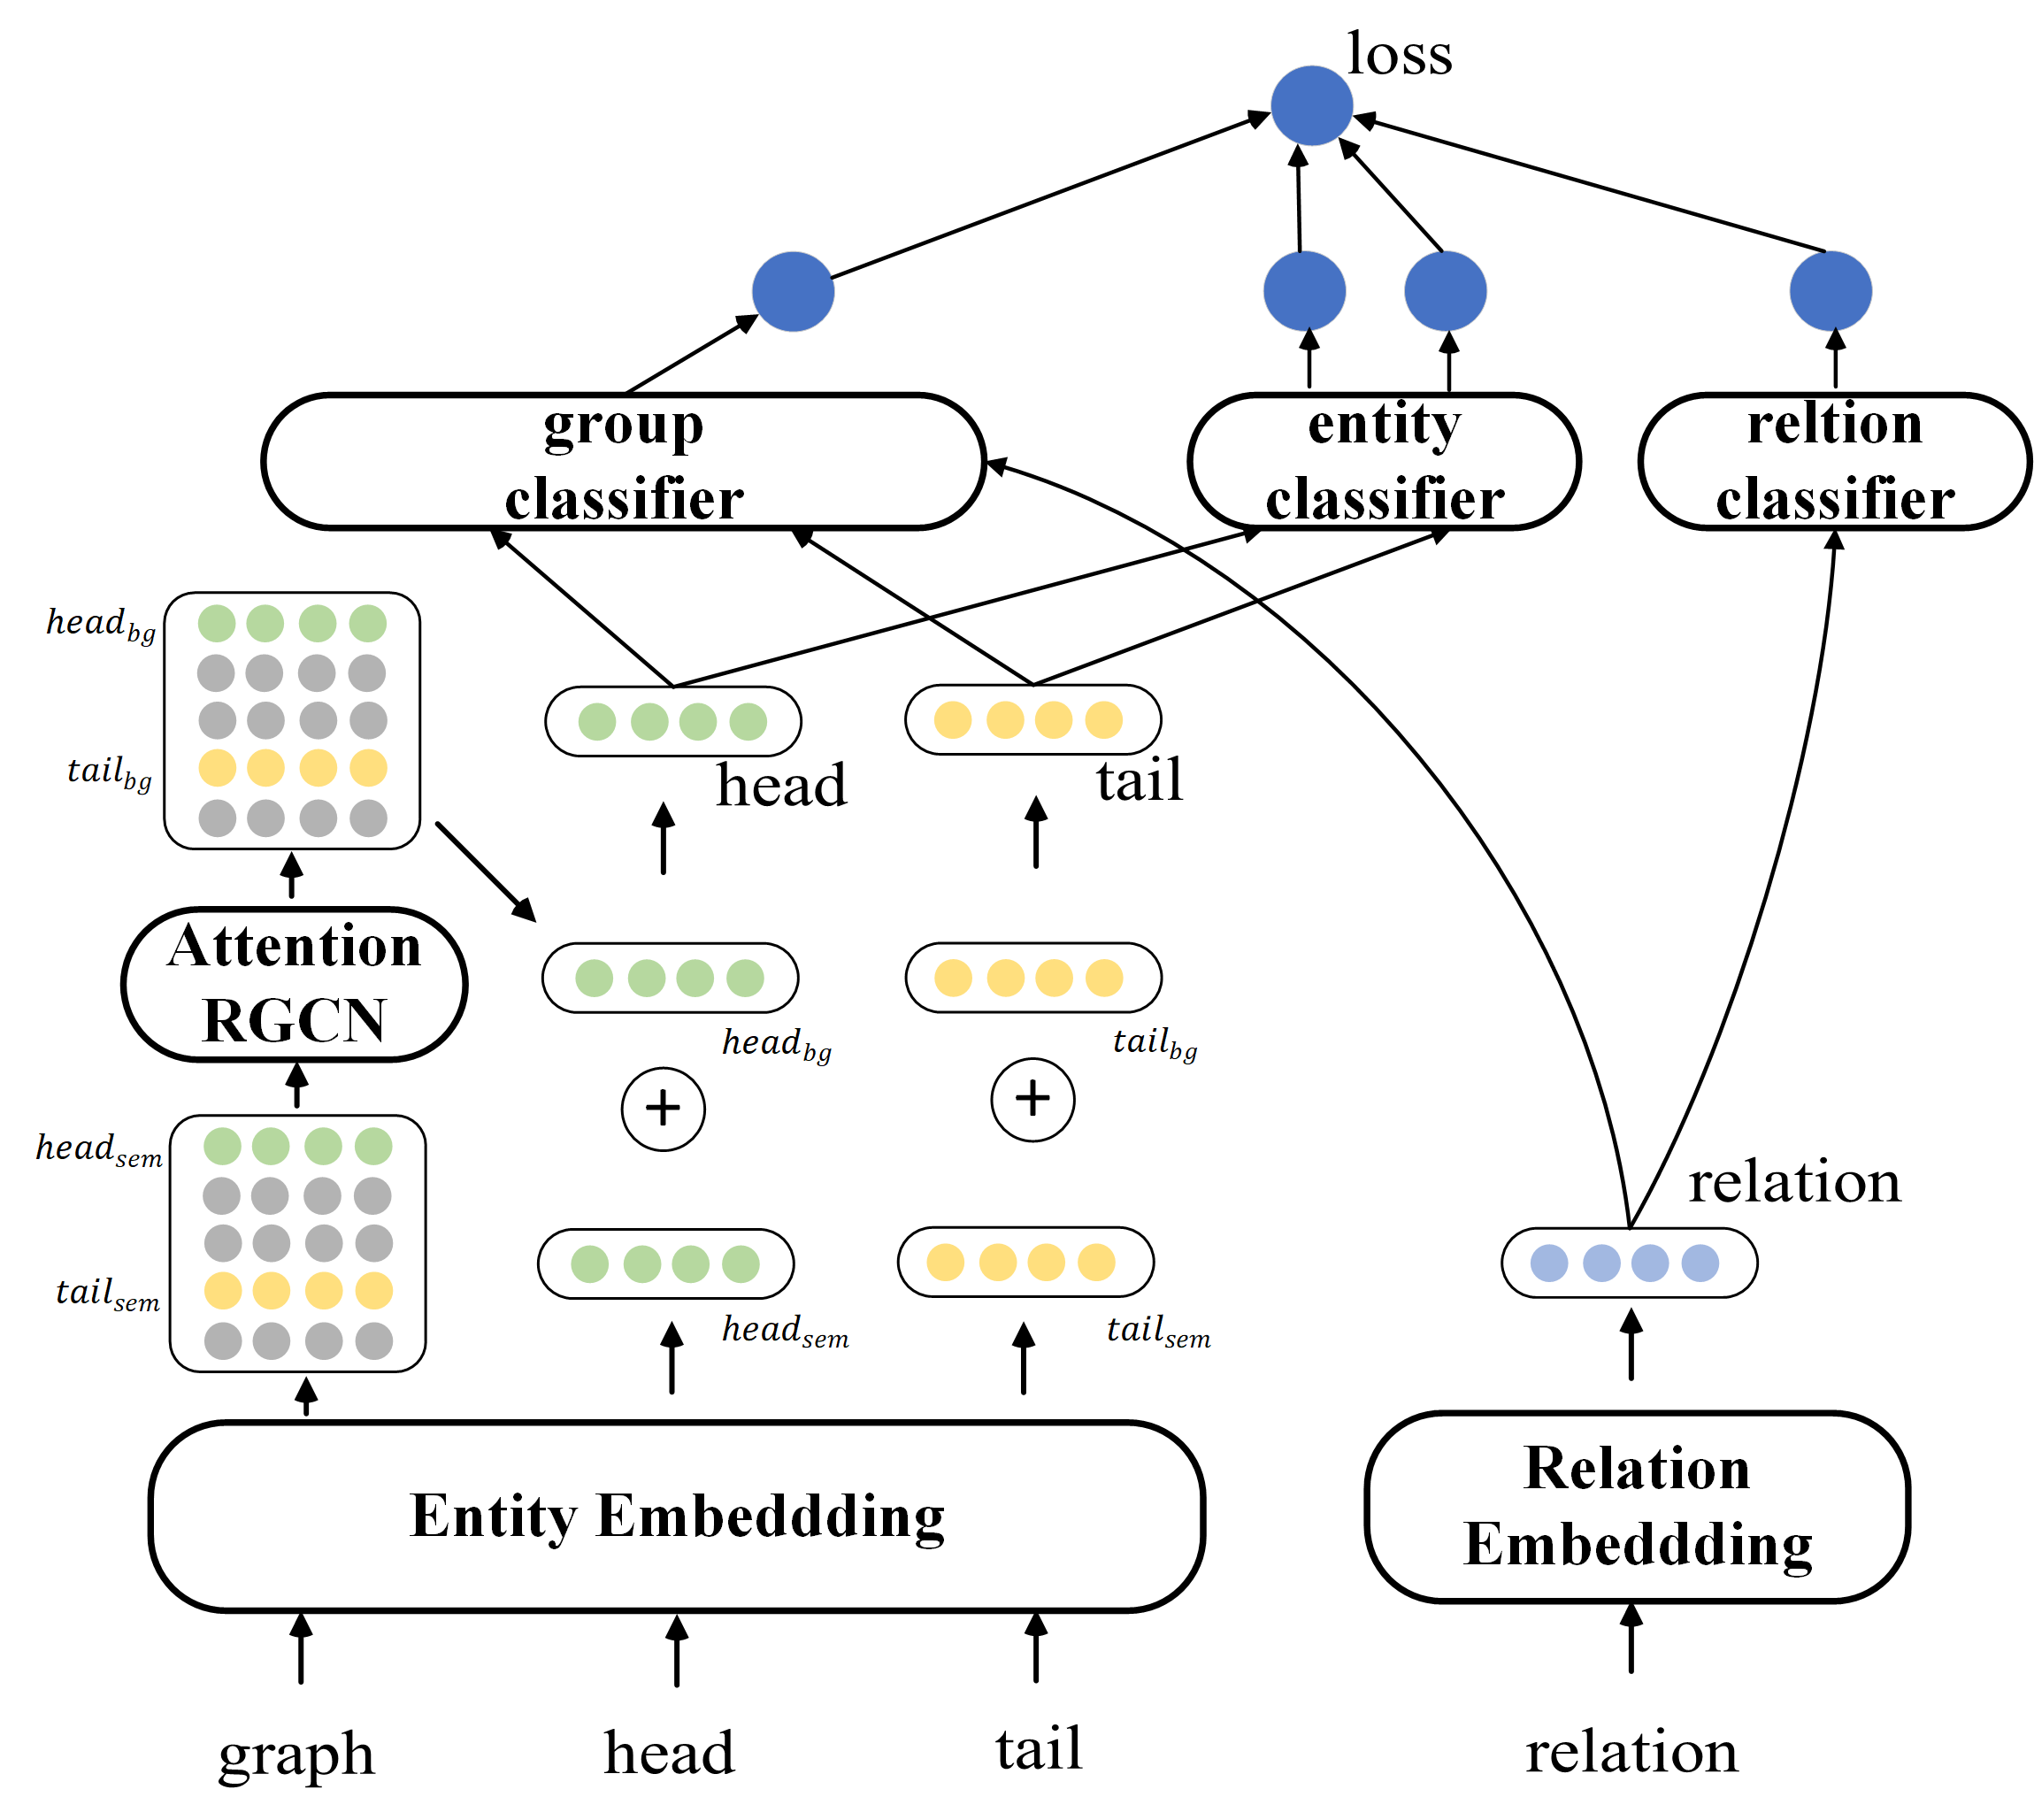
\includegraphics[width=.7\textwidth]{kg-representation.png}
    \caption{组件-事件知识图谱表示学习模型\label{kg-representation}}
\end{figure}

嵌入层:模型的输入除了三元组$(head, relation, tail)$还有该三元组所在的上下文图$graph$,即$(graph, head,rlation,tail)$。首先数据被输入embedding层转化为初步的嵌入表示,$graph$转为了张量矩阵,$head$、$relation$、$tail$则都被转为了单维的向量。初始的嵌入层向量来自于实体、关系的语义信息。具体实现上,使用文本类的日志数据对Bert\cite{devlin2018bert}进行预训练,然后每个实体或关系的初始特征向量使用其分词后多个单词的向量均值。

Attention-RGCN层:\ref{RGCN}已经对RGCN进行了介绍,在进行特征传播时,实体对其上下文实体都赋予了相同的权重。但在组件-事件知识图谱中,实体对其上下文邻居实体是有不同侧重的,如图\ref{graph-example}中$cpu 100\%$和$memory 100\%$导致了$Backoff$的发生,但$memory 100\%$对$Backoff$的发生更具关键性,它意味着$container1$中没有足够的内存满足$ts-train-service$的启动需求。因此,本文将注意力机制引入图卷积网络的传播过程,如式子\ref{attention-rgcn}所示。
\begin{equation}
    h_{i}^{(l+1)}=\sigma\left(\sum_{r \in \mathcal{R}} \sum_{j \in \mathcal{N}_{i}^{r}} \alpha_{(j, r, i)} \frac{1}{c_{i, r}} W_{r}^{(l)} h_{j}^{(l)}+W_{0}^{(l)} h_{i}^{(l)}\right)
    \label{attention-rgcn}
\end{equation}
整体结构与式\ref{propo-in-directedgraph}一致,其中新引入的$\alpha_{(j, r, i)}$目的在于计算第$i$个结点对其在关系$r$下的所有邻居结点$j \in \mathcal{N}_{i}^{r}$的注意力权重。其计算公式如下:
\begin{equation}
    v_{(j, r, i)}=\mathbf{a}^{T}\left[\mathbf{W} h_{j}\left\|\mathbf{W} h_{r}\right\| \mathbf{W} h_{i}\right]
    \label{group-loss-part1}
\end{equation}
\begin{equation}
    \alpha_{(j, r, i)}=\operatorname{softmax}\left(v_{(j, r, i)}\right)=\frac{\exp \left(v_{(j, r, i)}\right)}{\sum_{j^{\prime} \in \mathcal{N}_{i}^{r}} \exp \left(v_{\left(j^{\prime}, r, i\right)}\right)}
    \label{group-loss-part2}
\end{equation}
式\ref{group-loss-part1}中$h_i,h_j,h_r\in\mathbb{R}^{d}$,$\mathbf{W} \in \mathbb{R}^{d\times d}$是共享的参数矩阵。$\mathbf{a} \in \mathbb{R}^{3 d}$是权重向量,$\|$为向量级联操作。最终得到的$ v_{(j, r, i)} \in \mathbb{R}$即为索引为$i$的结点对关系$r$下索引为$j$的结点的注意力权重值。式\ref{group-loss-part2}使用$softmax(.)$函数进一步规范化注意力权重值,其中$\mathcal{N}_{i}^{r}$为索引为$i$的结点在关系$r$下对应的实体索引值集合。经过Attention-RGCN层后可以得到$head$、$tail$对应的上下文图结构嵌入表示$head_{bg}$、$tail_{bg}$,再与通过初步embedding层的语义向量累加即可得到$head_{sem}$、$tail_{sem}$同时融入了语义信息和上下文图结构信息的嵌入表示$head_{new}$、$tail_{new}$。

实体分类器:对实体进行分类,类别标签包括$contanier$、$event$、$service$等共计$c_{n}$个。输入为经过attention-RGCN得到的融合了语义及上下文图结构信息的嵌入表示$head_{new}$、$tail_{new}$。随后将$head_{new}$、$tail_{new}$输入$d \times c_{n}$的$softmax(.)$层即可,即可得到实体对各类分类情况。损失函数使用交叉熵,如式\ref{my_entity_loss}所示。其中,$i$、$j$对应着$head$、$tail$两实体的索引号,$h_i$、$h_j$为两实体在网络模型中的输出,$y_i$、$y_j$为两实体的标注向量,$k$表示向量第$k$维度。
\begin{equation}
    \mathcal{L}_{entity}= - \sum_{k=1}^{K} y_{i k} \ln h_{i k} - \sum_{k=1}^{K} y_{j k} \ln h_{j k}
    \label{my_entity_loss}
\end{equation}

关系分类器:对关系向量分类,类别包括$cause$、$happen$、$hold$等。与实体分类一样,使用$softmax(.)$层分类,然后损失函数使用交叉熵即可,如式\ref{my_relation_loss}所示。其中,$h_r$为关系对应的网络输出向量,$y_r$为关系的标注向量,$k$表示向量第$k$维度。
\begin{equation}
    \mathcal{L}_{relation}=- \sum_{k=1}^{K} y_{r k} \ln h_{r k}
    \label{my_relation_loss}
\end{equation}

三元组分类器:判别三元组是否存在。可以使用文献\parencite{trouillon2016complex}中形如式\ref{attention-rgcn-group-score}的评分函数。其中$\operatorname{diag}\left(.\right)$将$h_r\in\mathbb{R}^{d}$中每一个元素当作二维矩阵的对角线元素,从而得到$\mathbb{R}^{d}\times \mathbb{R}^{d}$的二维矩阵。损失函数使用交叉熵,如式\ref{my_group_loss}所示,其中$\mathcal{T}$表示所有的输入$(g, i, r, j)$集合,$l(.)$为激活函数,$y$为三元组是否成立的标签。
\begin{equation}
    f(h_{j}, h_{r}, h_{i})=h_{j}^{T} \operatorname{diag}\left(h_{r}\right) h_{i}
    \label{attention-rgcn-group-score}
\end{equation}

\begin{equation}
    \mathcal{L}_{group}= -\frac{1}{|\mathcal{T}|}  \sum_{(g, i, r, j) \in \mathcal{T}} y \log l(f(h_i, h_r, h_j))+(1-y) \log (1-l(f(h_i, h_r, h_j)))
    \label{my_group_loss}
\end{equation}

\subsection{参数学习}\label{representation-paras-learn}
根据上一小节所述,本模型的损失函数为实体分类器、关系分类器、三元组分类器三部分损失函数之和。最终本模型的损失函数如式\ref{represent-loss-all}所示:

\begin{equation}
    \begin{aligned}
    \mathcal{L}=-\frac{1}{|\mathcal{T}|}&  \sum_{(g, i, r, j) \in \mathcal{T}} y \log l(f(h_i, h_r, h_j))+(1-y) \log (1-l(f(h_i, h_r, h_j)))\\
    &- \sum_{k=1}^{K} y_{i k} \ln h_{i k} - \sum_{k=1}^{K} y_{j k} \ln h_{j k}\\
    &- \sum_{k=1}^{K} y_{r k} \ln h_{r k}\\
    \end{aligned}
    \label{represent-loss-all}
\end{equation}

\subsection{预测}
对组件-事件知识图谱进行表示学习后,可以进行抽象事件预测(预测在已发生抽象事件情况下是否会在某组件上发生某种事件)。根本上,就是在给定上下文图结构$g$下,三元组$(i, r, j)$是否成立。

将上下文图结构、头实体、关系和候选尾实体$g$、$(i, r, j)$输入表示学习模型中,会得到该三元组成立的评分,将评分最高的三元组对应的尾实体作为预测事件即可,如式\ref{predict-next-event}所示。

\begin{equation}
    e = \mathop{\arg\max}\limits_{j\in events}( f (h_i, h_r, h_j)) 
    \label{predict-next-event}   
\end{equation}


\section{本章小结}
本章主要介绍了组件-事件知识图谱的表示学习模型,通过将实体表示分为结构特征和语义特征,其中拓扑结构通过图卷积网络获取,语义特征使用实体分词对应词向量均值表示,从而实现了实体在不同拓扑上下文的动态表示,另外也介绍了参数更新和预测事件的公式。下一章将在本章提出的表示学习模型基础上进行故障预测。

% 1、基于 h r t 三元组
% 相关工作:基于path的那种
% 本文:将上下文考虑进去,上下文要么 (hrt)集合  要么图(ve)
% loss:分类,三元组判别对不对
% 评判标准:链路预测、实体分类

% 2、基于 网络表示学习 的那种
% 相关工作:基于rgcn的那种
% 本文:将上下文考虑进去,上下文要么 (hrt)集合  要么图(ve)
% loss:分类,三元组判别对不对
% 评判标准:关系预测、结点分类



